\documentclass[12pt, a4paper, openany]{book}
\usepackage{../generalStyle}

\graphicspath{ {./img/} }
\renewcommand{\labelenumii}{\arabic{enumi}.\arabic{enumii}}

\begin{document}
\title{LC - Linguaggi e Computabilità}
\author{Elia Ronchetti\\
    \small{\href{https://t.me/ulerich}{@ulerich}}}
\date{Settembre 2022}

\maketitle
\tableofcontents

\chapter{Linguaggi formali}
Preso un alfabeto $\Sigma=\{a,b,c\}$ posso formare delle stringhe come
\\ $\{bab, aca, b\}$, questo insieme è un linguaggio sull'alfabeto $\Sigma$.
\\ Con un linguaggio posso fare principalmente 2 cose
\begin{itemize}
    \item Riconoscitori - detti anche \textbf{automi}, sono degli automi che prendono in input
    una stringa e mi dicono se appartiene o no al linguaggio, \textbf{riconoscono} quindi il linguaggio
    \item Generatori - sono le Grammatiche, dalla grammatica posso generare il linguaggio,
    esse mi danno diverse regole attraverso le quali posso generare un linguaggio.
\end{itemize}
\paragraph*{Alfabeto} Un alfabeto è un insieme non vuoto e finito di simboli
\definizione{Un alfabeto è un insieme non vuoto e finito di simboli
definito con la lettera $\Sigma$}
\esempio{$\Sigma = \{0,1\}$}
\definizione{Una \textbf{stringa} è una sequenza finita di simboli dell'alfabeto.
    \\ In questo caso è ammesso l'insieme vuoto, si parla di stringa vuota e viene definita
    come $\epsilon$
    \begin{center}
        $L \subseteq \Sigma^*$
    \end{center}
}
La lunghezza di una stringa viene denotata dai seguenti simboli $|\text{stringa}|$.
\esempio{$|0111|=4$}
$\Sigma^n$ è una stringa di lunghezza.
\definizione{Un \textbf{Linguaggio} (su un alfabeto $\Sigma$ è un sottoinsieme di $\Sigma^*$)}
\paragraph*{Notazioni particolari}
\begin{itemize}
    \item $\Sigma^0 = \{\epsilon\}$
    \item $\Sigma^* = \Sigma^0 \cup \Sigma^1 \cup ...$ oppure $\Sigma^*=\Sigma^+ \cup \Sigma^0 = \Sigma^+ \cup \{\epsilon\}$
    \item $\Sigma^+ = \Sigma^1 \cup \Sigma^2 \cup \Sigma^3 \cup ...$ oppure $\Sigma^+ = \Sigma^* - \{\epsilon\}$
\end{itemize}
\paragraph*{Notazioni stringhe} Per definire una stringa utiizzo una lettera come per esempio
$w = abb$ dove in w sono contenuti dei simboli dell'alfabeto $\Sigma=\{a,b,c\}$.
\\ Definita un'altra stringa $y=cca$ definisco la concatenazione di due stringhe come $wy = abbcca$.
La concatenazione \textbf{NON} è commutativa.
\chapter{Le Grammatiche}
Una grammatica è una quadrupla
\begin{equation*}
    G=(V, T, P,S)
\end{equation*}
Dove
\begin{itemize}
    \item V è l'insieme delle Variabili
    \item T è l'insieme dei simboli Terminali
    \item P è l'insieme delle regole di Produzione
    \item S $\in$ V, è lo Start symbol
\end{itemize}
\definizione{Grammatica: termine che designa una struttura formale per un linguaggio L in grado di generare tutte e sole le stringhe del linguaggio.
    Per questo si parla di grammatica G generativa del linguaggio L o di linguaggio L generato dalla grammatica G, indicandolo con L(G).}
\textit{Definizione Treccani} \href{https://www.treccani.it/enciclopedia/grammatica_%28Enciclopedia-della-Matematica%29/}{Link alla definizione}
\section{Gerarchia di Chomsky}
La gerarchia di Chomsky è un insieme di classi di grammatiche formali che generano linguaggi formali.
Suddivide le grammatiche in 4 tipi:
\begin{itemize}
    \item Tipo 0 - Linguaggi ricorsivamente enumerabili
    \item Tipo 1 - Linguaggi Contestuali
    \item Tipo 2 - Linguaggi Context-Free (Liberi dal contesto)
    \item Tipo 3 - Linguaggi Regolari
\end{itemize}
\subsection{Tipo 0}
Sono definiti nel seguente modo:
\begin{center}
    $\alpha \rightarrow \beta$, con $\alpha$ e $\beta \in (V \cup T)^*$
\end{center}
\esempio{$0S1S0 \rightarrow 00SS1S01$}
Sono detti \textbf{ricorsivamente enumerabili} e vengono accettati dalle 
\textbf{Macchine di Turing deterministiche e non deterministiche}.
\subsection{Tipo 1}
Verranno solo visti un paio di esempi, ma non saranno trattati in questo corso.
\\ Definiti nel seguente modo:
\begin{center}
    $\alpha_1 \, A \, \alpha_2 \rightarrow \alpha_1 \, \beta \, \alpha_2$
    \\ $A\in V \qquad \alpha_1, \alpha_2, \beta \in (V \cup T)^*$
\end{center}
In questo linguaggio sono presenti più vincoli rispetto al tipo 0.
Questi linguaggi sono detti contestuali, questo perchè posso sostituire le variabili solo in un determinato contesto, in questo caso
solo se sono presenti sia $\alpha_1$ e $\alpha_2$ tra $\beta$.
\\ Sono accettati dalle \textbf{Macchine di Turing con nastro "lineare"}.
\subsection{Tipo 2}
$A\rightarrow \gamma \qquad A \in V$, $\gamma \in \, (V \cup T)^*$.
\\ Detti anche \textbf{Context-Free (Liberi dal Contesto)}.
\\ Riconosciuti da \textbf{Automi a Pila non deterministici}
\subsection{Tipo 3}
$A \rightarrow aB$ oppure $A \rightarrow a$ oppure
\\ $A \rightarrow Ba$ oppure $A \rightarrow a$.
\\Sono detti \textbf{Regolari} e sono riconosciuti da \textbf{Automi
a stati finiti deterministici e non deterministici}.

\paragraph*{Osservazione}Scorrendo verso il basso la gerarchia noto che le grammatiche sono sempre più
stringenti e meno libere.

\subsection*{Produzione di un linguaggio}
Per produrre un linguaggio è necessario definire la relativa grammatica (V, T, P, S).
Quando scrivo le regole di produzione non posso imporre un ordine di applicazione delle regole e non posso
negare l'applicazione di una regola, tutte le regole possono essere applicate in qualsiasi ordine.
\paragraph*{Regole di Produzione} Con regole di produzione si intendono le regole che mi permettono di passare
da una variabile ad un simbolo per poter costruire una frase.
\esempio{Bilanciamento parentesi
\\ $G_bal = \{\{S\},\{(,)\}, P, S\}$
\\ P$\{S\rightarrow SS | (S) | \epsilon\}$
\\ In questo caso la freccia indica una regola di produzione
\\ Esempi di frasi valide $\rightarrow (), (()),()()$
\\ Esempi di frasi non appartenentei al linguaggio $\rightarrow )($
\\ \emph{Applicazione regole di produzione}
\\ $S \Rightarrow \underline{S}S \Rightarrow (S)\underline{S} \Rightarrow (S)(\underline{S})
\Rightarrow(\underline{S})() \Rightarrow ((\underline{S}))()\Rightarrow(())()$
\\ Sostituendo i le variabili attraverso le regole di produzione ottengo le frasi appartenenti
al linguaggio.
\\ \emph{In questo caso $\Rightarrow$ indica un passaggio di derivazione}}
\paragraph*{Attenzione} Non si effettuano mai più sostituzioni in un unico passaggio,
dato che non è garantito che il risultato ottenuto sia corretto.
\\ Con $\Rightarrow^*$ indico che faccio uno o più passi di derivazione (NON più sostituzioni in un unico
passaggio).
\section{Context Free Grammar (CFG) - Linguaggi liberi dal contesto (Tipo 2)}
Questi linguaggio sono caratterizzati da una definizione ricorsiva dello stesso, qui di
seguito alcuni esempi per chiarire cosa si intende.
\esempio{\emph{Fornire una CFG per il linguaggio $L=\{0^n 1^n | n \geq 1\} n\in \mathbb{N}$}
Alcuni esempi di L sono = \{01, 0011, 000111, ...\}
\\ Se $w in L$ allora $0w1 \in L$
\\ $S \rightarrow 01 | 0S1$
\\ $V = \{S\},\, T=\{0,1\}$ $G = (V,T,P,S)$
\\ $S \Rightarrow 0S1 \Rightarrow 00S11 \Rightarrow 000111$
\\ \emph{n ci indica quante volte il simbolo si deve ripetere come minimo, in questo caso per
esempio essendo $\geq 1$ ci sta dicendo che vuole che il simbolo sia ripetuto almeno 1 volta, quindi
$\epsilon$ non è ammesso, fosse stato $\geq 0$ significava che $\epsilon$ appartiene al linguaggio}}
\subsection*{Left Most e Right Most derivation}
Posso applicare le regole di derivazione in diversi ordini, per esempio applicando sempre la variabile più
a sinistra o più a destra, vedremo che questo non cambia il risultato, disegnando un albero sintattico noteremo
come i due rami a seconda del tipo di applicazione risulteranno invertiti, ma il risultato sarà sempre lo stesso.
\subsection*{Risoluzione esercizi}
Lo svolgimento degli esercizi è sui PDF presenti nella cartella drive indicata nel README.md, comunque
qui di seguito sono elencati consigli per la risoluzione.
\paragraph*{Incroci} Nelle CFG non possono esserci "incroci" fra esponenti uguali, come per esempio
\esempio{$a^n b^m c^n y^m$} In questo caso le n e m risultano incrociate, non posso suddividerle in pattern o
sottopattern e questo mi impedisce di produrre una CFG.
\begin{itemize}
    \item Ragionare sul pattern delle lettere e non sulla singola lettera
    \item Partire dall'esterno e mano a mano passare ai pattern più interni per creare le regole di produzione
    \item Per ogni pattern identificato sarà necessario utilizzare una Variabile
    \item Quando ho situzioni di questo tipo $a^{n+m}xc^n y d^m$ è necessario prestare attenzione a
    come si dividono i due esponenti perchè a volte posso generare degli incroci, per questo è necessario
    scomporre l'esponente nell'ordine corretto, quello che mi permette di ottonere gruppi non incrociati
    \item La situazione precedente tipicamente si presenta negli esercizi dove come condizioni ho $n \geq m \geq 0$
\end{itemize}

\section{Linguaggi di Tipo 1 (Contestuali)}
%Iniziata trascrizione lezione 4 - Vedere PDF Grammatiche di Tipo 1 su elearning
% https://elearning.unimib.it/pluginfile.php/1366772/mod_resource/content/3/grammatiche-tipo-1.pdf
Le Grammatiche di Tipo 1 sono dipendenti dal contesto, questo significa che durante
la produzione di una stringa viene sostituito un simoblo alla volta, ma solo quando
è in presenza di un altro simbolo. Vedremo che nella testa delle regole di produzione
avrò la concatenazione di due variabili.
Nell'esempio riportato a questo 
{\href{https://elearning.unimib.it/pluginfile.php/1366772/mod_resource/content/3/grammatiche-tipo-1.pdf}{\textbf{link}}}
vengono mostrate le regole di produzioni necessarie per generare un esempio di linguaggio
di tipo 1. 

\section{La Grammatiche Ambigue}
\subsection{Albero Sintattico}
Data una CFG $G= (V,T,P,S)$ un modo per rappresentare le regole di produzione applicate è rappresentare l'albero sintattico.
Esso consiste in un alberto dove le foglie sono etichettate con una variabile, da un simbolo
terminale o da $\epsilon$. Ogni nodo interno è etichettato con una variabile, 
se è etichettato da $\epsilon$ è l'unica foglia del suo genitore.
\\ Qui di seguito un esempio di albero per la derivazione della stringa $iee$
\begin{center}
    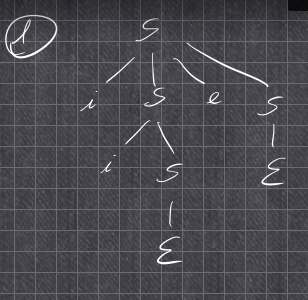
\includegraphics[width=50mm, scale=0.5]{albero_sintattico.png}
\end{center}
Se un nodo interno è etichettato con A e i figli sono etichettati da sinistra
con $X_1, X_2, ..., X_n$ allora $A \rightarrow X_1, X_2, X_k \in P$.
La definizione è importante per l'argomento che adesso andremo a trattare
\section*{Ambiguità}
Se una grammatica consente la generazione della stessa stringa attraverso due alberi sintattici
diversi allora quella è una grammatica ambigua.
\definizione{
    \begin{enumerate}
        \item $\exists w \in T^*$ tale che w ha due alberi sintattici diversi
        $rightarrow$ Grammatica Ambigua
        \item $\forall w \in T^*$ w ha un solo albero sintattico $\rightarrow$
        Grammatica NON Ambigua 
    \end{enumerate}
}
\paragraph*{NB} Ottenere la stessa stringa con derivazioni diverse non è un problema,
il problema è quando ottengo \textbf{Alberi sintattici diversi!}.
Se una Grammatica è ambigua posso risolvere il problema e renderla non ambigua, mentre
se un linguaggio è ambiguo NON posso risolvere il problema dato che
un linguaggio ambiguo può essere generato solo da Grammatiche ambigue.
\paragraph*{Problema} Non esiste un algoritmo in grado di identificare una grammatica
ambigua. Gli esempi pratici li trovate nelle ultime pagine di questo PDF - 
{\href{https://drive.google.com/drive/folders/1gdH43dnEfCeLGmq08HEBwQoKORGgcQdY}{\textbf{Lezione 4}}}.
\section{Grammatiche Regolari (Tipo 3)}
\begin{enumerate}
    \item \eps può comparire solo in $S \rightarrow \epsilon$, dove S è lo start symbol
    \item le regole di produzione sono tutte lineari a destra oppure tutte lineari a sinistra
\end{enumerate}
\esempio{Lineare a Destra
\\ $A \rightarrow aB
\\ A \rightarrow a$ dove $A,B \in V$ $a \in T$ }
\esempio{Lineare a Sinistra
\\ $A \rightarrow Ba
\\ A \rightarrow a$ dove $A,B \in V$ $a \in T$}
Non si possono mischiare questi due esempi, o sono lineare a sinistra o a destra.
\chapter{Espressioni Regolari}
\definizione{Un'espressione regolare (in lingua inglese regular expression o, in forma abbreviata, regexp, regex o RE) 
è una sequenza di simboli (quindi una stringa) che identifica un insieme di stringhe.
Possono definire tutti e soli i linguaggi regolari.}
\section{Operazioni Tra Linguaggi}
\subsection*{Unione}
Dati $L,M \rightarrow L \cup M$
\esempio{L = \{001, 10,111\}
\\ M = \{\eps, 001\} 
\\ L $\cup$ M = \{\eps, 001, 10, 111\}}
Gli elementi in comune non si ripetono
\subsection*{Concatenazione} $L,M \rightarrow LM$
\esempio{L = \{001, 10, 111\}
\\ M = \{\eps, 001\}
\\ LM = \{001, 001001, 10, 10001, 111, 111001\}}
Tutte le possibili concatenazioni
\subsection*{Chiusura di Kleene} $L = \emptyset$
\esempio{$\emptyset^0 = \{\epsilon\}
\\L^0 = \{\epsilon\}\forall L
\\ \emptyset^i = \emptyset \forall_i \geq 1
\\ \emptyset^* = \emptyset^0 \cup \emptyset^1 \cup \emptyset^2 \cup \dots =
\\ \{\epsilon\} \cup \emptyset \cup \emptyset \cup \dots =
\\ \{\epsilon\}$}
\section*{Espressioni Regolari}
\paragraph*{NB} In questo contesto \eps e $\emptyset$ sono ER (Espressioni
Regolari) NON sono stringhe.
\begin{enumerate}
    \item \eps e \empt sono ER \ra L(\eps) = \{\eps\} L(\empt) = \empt
    \item Se $a \in \Sigma$ allora a è una ER (Dove $\Sigma$ è alfabeto)
    \item Variabili che rappresentano linguaggi sono ER
\end{enumerate}
\paragraph*{Induzione}
\begin{enumerate}
    \item \textbf{Unione} \ra se E,F sono ER allora E+F è una ER \\
    $L(E+F) = L(E)\cup L(F)$
    \item \textbf{Concatenazione} \ra se E,F sono ER allora EF è una ER \\
    $L(EF) = L(E)*L(F)$
    \item \textbf{Chiusura} \ra Se E è ima ER allora E* è una ER \\
    $L(E^*) = (L(F))^*$
    \item \textbf{Parentesi} \ra Se E è una ER allora (E) è una ER \\
    $L((E)) = L(E)$
\end{enumerate}
\paragraph*{Proprietà}
\begin{itemize}
    \item \textbf{Unione} \ra Commutativa, Associativa \\
    $L+M = M+L$ \\ $(L+M)+N = L+(M+N) = L+M+N$
    \item \textbf{Concatenazione} \ra Associativa, NON è commutativa \\
    $(LM)N=L(MN)$ \\ $01 \neq 10$
\end{itemize}
%Finito Lezione 6 - Iniziare Lezione 7 (Proprietà Algebriche ER)
\end{document}